\section{Metodologia}

\subsection{Formulação do Problema de reconfiguração de Rede Elétrica}

\begin{figure}[h]
    \centering
    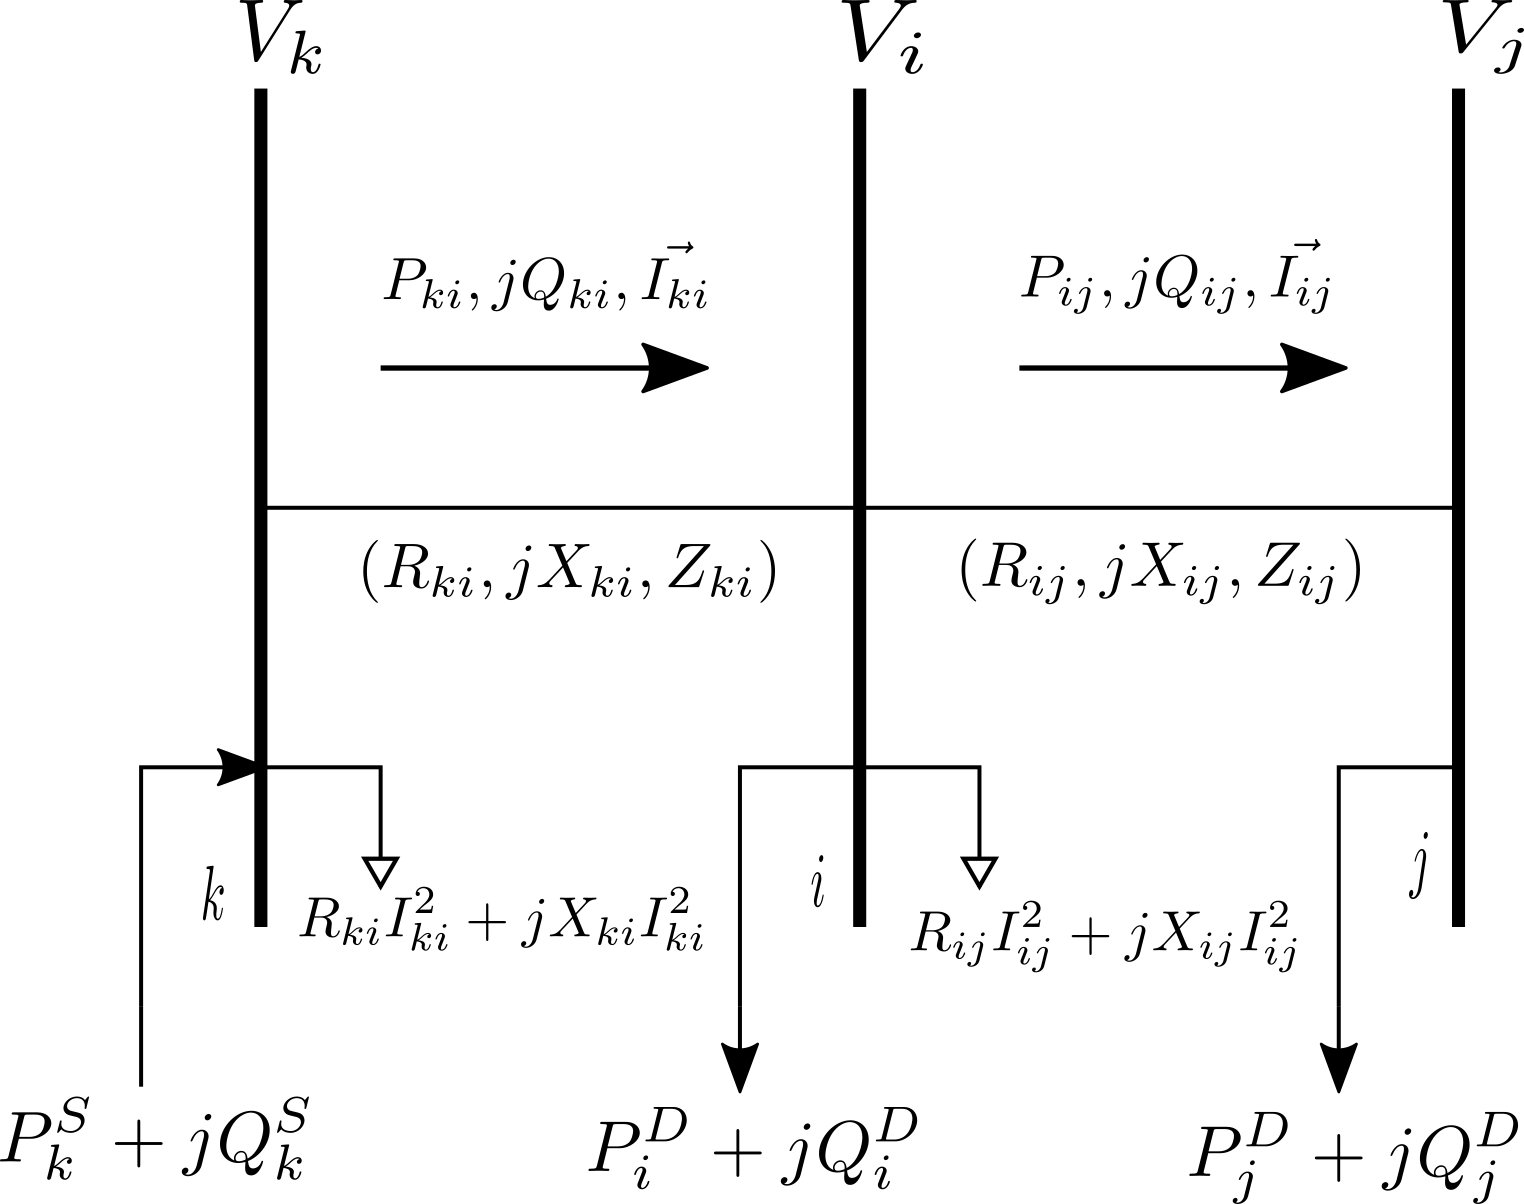
\includegraphics[]{01img/diagrama.png}
    \caption{Sistema de distribuição radial}
    \label{SDR}

\end{figure}

Hipóteses adotadas:

Visando representar o funcionamento em regime permanente de um sistema de distribuição de energia, são feitas as seguintes hipóteses (comumente usadas nas formulações de fluxo de carga varredura \cite{ShirmohammadiANetworks} e mostradas na figura \ref{SDR}.

\begin{itemize}
    \item As demandas nas cargas na rede de distribuição são representadas como potência ativa e reativas contantes;
    
    \item O sistema é balanceado e representado pelo seu equivalente monofásico;
    
    \item As perdas de potência ativa e reativa no circuito ij estão concentradas no nó i.
    
    \item As chaves são representadas como circuito curtos de impedância nula.
\end{itemize}

De acordo com a figura \ref{SDR}, os termos $\Vec{V}_{i}$ e $\Vec{I}_{ij}$ representam os fasores da tensão no nó i e a corrente que vai do nó i para o nó j, respectivamente. 
$P_{i}^{D}$ e $Q_{i}^{D}$ representam a potência ativa e reativa demandada no nó i, respectivamente.

Formulação do Problema de Fluxo de Carga para redes elétricas radiais:

Da figura \ref{SDR}, a queda de tensão do circuito é definida pela equação \ref{eq:queda_tensao}.

\begin{equation}
    \Vec{V}_{i} - \Vec{V}_{j} = I_{ij}(R_{ij} + jX_{ij})\quad\forall ij \in \Omega_{l}
    \label{eq:queda_tensao}
\end{equation}

Em que $\Omega_{l}$ é o conjunto de circuitos. %OBSERVAÇÃO: Explicar mais sobre o conjunto de circuitos
Através da fórmula para o cálculo da potência aparente, $I_{ij}$ pode ser calculado usando a equação \ref{eq:corrente_ramo}.

\begin{equation}
    I_{ij} = \left(\frac{P_{ij} + jQ_{ij}}{\Vec{Vj}}\right)^{*}\quad\forall ij \in \Omega_{l}
    \label{eq:corrente_ramo}
\end{equation}

%OBSERVAÇÃO: Explicar o uso da tensão Vj e as potências (Considerou-se que as perdas ao longo do ramo ij estão concentradas no nó i, por isso a potência que passa ao longo do ramo é a potência Sij que é igual a potência drenada do nó j

Substituindo $I_{}ij$ da equação \ref{eq:corrente_ramo} na e equação \ref{eq:queda_tensao} obtém-se a equação \ref{eq:queda_tensao_pot} que define a queda de tensão em função das potências e impedâncias do circuito.

Seja $(P_{ij} + jQ_{ij})^{*} = (P_{ij} - jQ_{ij})$ logo:

\begin{equation}
    (\Vec{V}_{i} - \Vec{V}_{j})\Vec{V}_{j}^{*} = (P_{ij} - jQ_{ij})(R_{ij} + jX_{ij}) \quad\forall ij \in \Omega_{l}
    \label{eq:queda_tensao_pot}
\end{equation}

Considerando que $\Vec{V}_{i} = V_{i}\angle{\theta_{i}}$, $\Vec{V}_{j} = V_{j}\angle{\theta_{j}}$ e $\theta_{ij} = \theta_{i} - \theta_{j}$, tal que  $V_{i}$ e $V_{j}$ representam as magnitudes da tensão em seus respectivos nós bem como $\theta_{i}$ e $\theta_{j}$ representam seus ângulos.
Dessa forma a equação \ref{eq:queda_tensao_pot} pode ser escrita decompondo a fase de suas exponenciais, como mostra a equação \ref{eq:queda_tensao_sencos}.

\begin{equation}
    V_{i}V_{j}[cos\theta_{ij} + jsen\theta_{ij}] - V_{j}^{2} = (P_{ij} - jQ_{ij})(R_{ij} + jX_{ij}) \quad\forall ij \in \Omega_{l}
    \label{eq:queda_tensao_sencos}
\end{equation}

Identificando as partes real e imaginária na equação \ref{eq:queda_tensao_sencos}, obtém-se:

\begin{equation}
    V_{i}V_{j}cos\theta_{ij} = V_{j}^{2} + (R_{ij}P_{ij} + X_{ij}Q_{ij})\quad\forall ij \in \Omega_{l}
    \label{eq:queda_tensao_real}
\end{equation}

\begin{equation}
    V_{i}V_{j}sen\theta_{ij} = X_{ij}P_{ij} - R_{ij}Q_{ij}\quad\forall ij \in \Omega_{l}
    \label{eq:queda_tensao_imaginaria}
\end{equation}

Usando a fórmula da trigonometria, que é a relação básica entre o seno e o cosseno, $sen^{2}(\theta_{ij}) + cos^{2}(\theta_{ij}) = 1$, e somando os quadrados das equações \ref{eq:queda_tensao_real} e \ref{eq:queda_tensao_imaginaria}, obtém-se:

\begin{equation}
    V_{i}^{2} - 2(R_{ij}P_{ij} + X_{ij}Q_{ij}) - Z_{ij}^{2}I_{ij}^{2} - V_{j}^{2} = 0\quad\forall ij \in \Omega_{l}
    \label{eq:queda_tensao_restricao}
\end{equation}

Em que a magnitude do fluxo de corrente $I_{ij}$ é mostrado na equação \ref{eq:corrente_magnitude} calculado a partir do produto com seu complexo conjugado.

\begin{equation}
    I_{ij}^{2} = \frac{P_{ij}^{2}+Q_{ij}^{2}}{V_{j}^{2}}\quad\forall ij \in \Omega_{l}
    \label{eq:corrente_magnitude}
\end{equation}

Note que a equação \ref{eq:queda_tensao_restricao} não depende da diferença angular entre as tensões, e é possível obter a magnitude da tensão do nó ($V_j$) em termos da magnitude inicial ($V_i$), o fluxo de potência ativa ($P_{ij}$), o fluxo de potência reativa ($Q_{ij}$), a magnitude do fluxo de corrente ($I_{ij}$) e os parâmetros elétricos do ramo ij.  